\section{Theory of Operations}

\subsection{Introduction}
The \textbf{Timer} is a configurable timer module that supports a variety of timing functions,
including PWM generation and interrupt signaling. It features a counter that can be configured with a prescaler,
maximum count value, and PWM ceiling value.

\begin{figure}[h]
  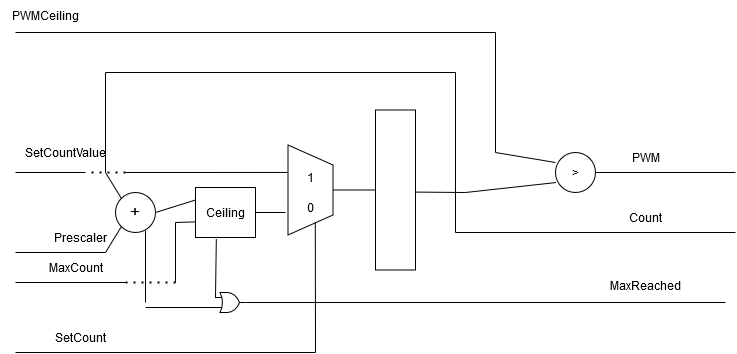
\includegraphics[width=0.80\textwidth]{images/TimerDragram.drawio.png}
  \caption{Timer Diagram}\label{fig:timer-diagram}
\end{figure}

The Timer module provides the following outputs:

\begin{itemize}[noitemsep]
  \item{\textit{count}: Current value of the counter.}
  \item{\textit{maxReached}: Signal indicating the counter has reached its maximum value.}
  \item{\textit{pwm}: PWM output signal with a duty cycle controlled by \textit{pwmCeiling}.}
  \item{\textit{interrupt}: Interrupt signal indicating timer events (e.g., max reached).}
\end{itemize}

\subsection{APB Interface}
The Timer module is accessed through an APB interface that can be be found
in the \href{https://github.com/The-Chiselers/apb}{APB Interface},
\href{https://github.com/The-Chiselers/registermap}{Register Map},
and \href{https://github.com/The-Chiselers/addrdecode}{Address Decoder} repositories.

\subsection{Organization}
The Timer module is divided into two sections: the TimerInner module which provides the core functionality,
and the Timer module that wraps the TimerInner module and provides the APB interface.

\subsection{Registers}
The Timer module provides the following registers:

\subsubsection{Inputs}
\begin{itemize}[noitemsep]
    \item{\textit{en}: Enable signal for the timer. When high, the timer is active.}
    \item{\textit{prescaler}: Prescaler value to divide the clock frequency.}
    \item{\textit{maxCount}: Maximum count value before the timer resets.}
    \item{\textit{pwmCeiling}: PWM ceiling value to control the duty cycle of the PWM signal.}
    \item{\textit{setCountValue}: Value to set the counter to when \textit{setCount} is asserted.}
    \item{\textit{setCount}: Signal to set the counter to \textit{setCountValue}.}
\end{itemize}

\subsubsection{Internal Registers}
\begin{itemize}[noitemsep]
    \item{\textit{prescalerCounter}: Counter to divide the clock frequency.}
    \item{\textit{prescalerWrap}: Signal indicating the prescaler has wrapped.}
    \item{\textit{countOverflow}: Signal indicating the counter has reached its maximum value.}
\end{itemize}

\subsubsection{Outputs}

\begin{itemize}[noitemsep]
    \item{\textit{count}: Current value of the counter.}
    \item{\textit{maxReached}: Signal indicating the counter has reached its maximum value.}
    \item{\textit{pwm}: PWM output signal with a duty cycle controlled by \textit{pwmCeiling}.}
    \item{\textit{interrupt}: Interrupt signal indicating timer events (e.g., max reached).}
\end{itemize}

\subsection{Enable and Reset}
When the timer module is not enabled, the inputs can all be programmed,
and the counter can be programmed as well but will not increment.
When the timer is enabled, the counter will increment on each clock cycle.